\title{Very Simple CPU\\(from \emph{Computer Systems Organization and Architecture}, by Carpinelli)}
\begin{document}
\section{Programing Model}

\begin{frame}{Fetch, decode, execute}
  Practically every CPU consists of a synchronous state machine that can be simplified to three states:
  \begin{itemize}
    \item Fetch
    \item Decode
    \item Execute
  \end{itemize}
  These three states can be broken down into substates to perform their tasks.
\end{frame}

\begin{frame}{Instructions and data}
  A CPU deals with two entities.
  \begin{itemize}
    \item Instructions
    \item Data
  \end{itemize}
  But remember, instructions are data too.
\end{frame}

\begin{frame}{Programming model}
  \begin{definition}
    The \alert{programming model} describes the registers and instructions that are available to the programmer.
  \end{definition}
  \begin{itemize}
    \item 1 register (AC - accumulator) (8 bit)
    \item 6 bit addressing (AR - address register) (PC - program counter)
    \item 1 internal data register (DR - data register) (8 bit)
    \item 2 bit instruction decoder (IR - instruction register)
    \item 4 instructions - ADD, AND, JMP, INC
  \end{itemize}
\end{frame}

\begin{frame}{Instructions}
  \begin{block}{Instruction format}
    Each instruction is 8 bits, 2 bits of opcode, 6 bits of argument (data).
  \end{block}
  \begin{tabular}{ccc}
    \textbf{Instruction} & \textbf{Code} & \textbf{Operation} \\
    \hline
    ADD & 00AAAAAA & AC $\leftarrow$ AC + M[AAAAAA] \\
    AND & 01AAAAAA & AC $\leftarrow$ AC $\cdot$ M[AAAAAA] \\
    JMP & 10AAAAAA & PC $\leftarrow$ AAAAAA \\
    INC & 11XXXXXX & AC $\leftarrow$ AC + 1
  \end{tabular}
\end{frame}

\section{Datapaths}

\begin{frame}{Datapaths}
  \begin{center}
    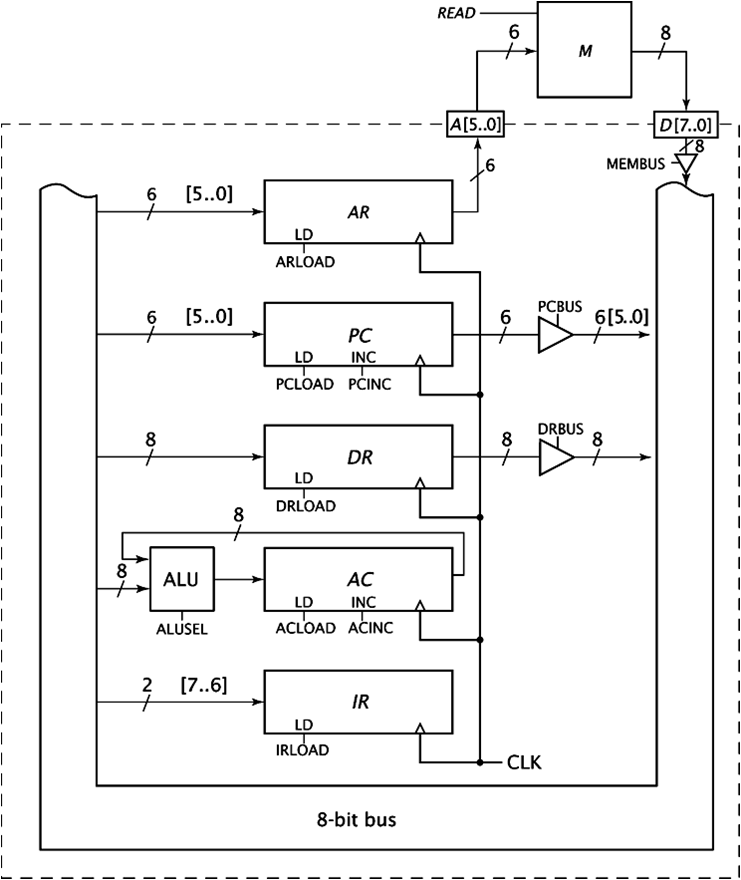
\includegraphics[scale=0.4]{DataPaths}
  \end{center}
\end{frame}

\begin{frame}{State diagram}
  \begin{center}
    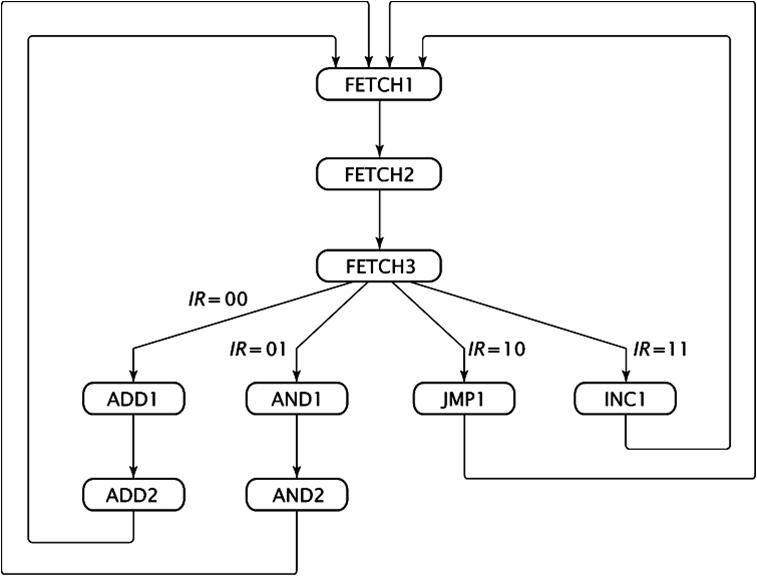
\includegraphics[scale=0.4]{StateDiagram}
  \end{center}
\end{frame}

\begin{frame}{Fetch and decode}
  We can describe each fetch state using register transfer language.
  \begin{itemize}
    \item FETCH1: AR $\leftarrow$ PC
    \item FETCH2: DR $\leftarrow$ M, PC $\leftarrow$ PC + 1
    \item FETCH3: IR $\leftarrow$ DR[7..6], AR $\leftarrow$ DR[5..0]
  \end{itemize}
\end{frame}

\begin{frame}{Instructions}
  \begin{itemize}
    \item Add
    \begin{itemize}
      \item ADD1: DR $\leftarrow$ M
      \item ADD2: AC $\leftarrow$ AC + DR
    \end{itemize}
    \item And
    \begin{itemize}
      \item AND1: DR $\leftarrow$ M
      \item AND2: AC $\leftarrow$ AC $\cdot$ DR
    \end{itemize}
    \item Jmp
    \begin{itemize}
      \item JMP1: PC $\leftarrow$ DR[5..0]
    \end{itemize}
    \item Inc
    \begin{itemize}
      \item INC1: AC $\leftarrow$ AC + 1
    \end{itemize}
  \end{itemize}
\end{frame}

\begin{frame}{Detailed datapaths}
  \begin{center}
    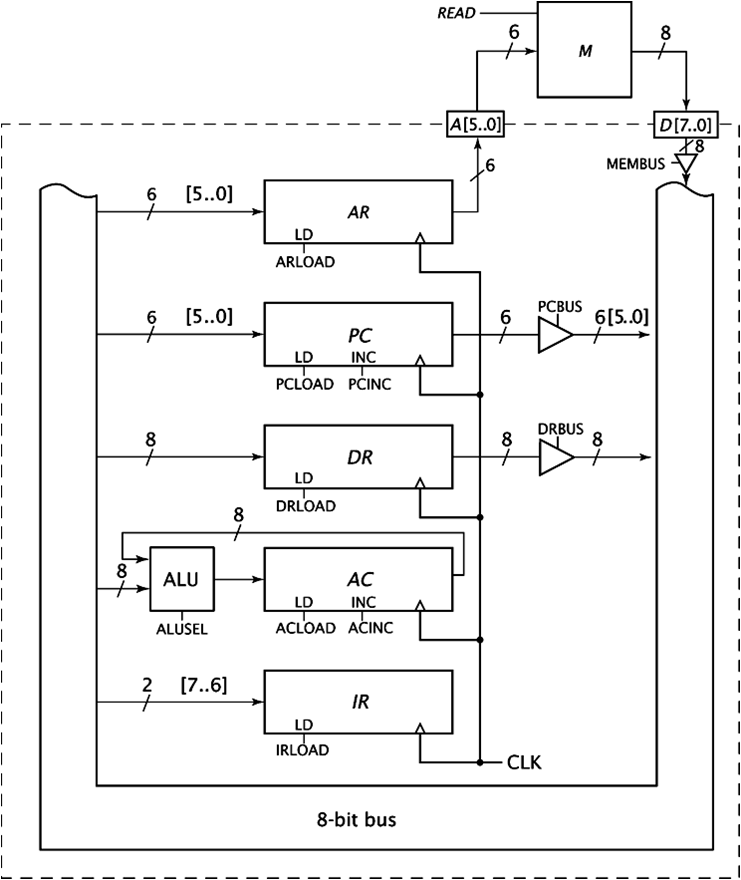
\includegraphics[scale=0.4]{AdvancedDataPaths}
  \end{center}
\end{frame}

\begin{frame}{ALU}
  \begin{center}
    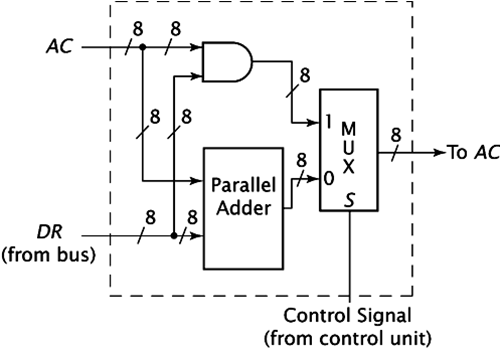
\includegraphics[scale=0.4]{ALU}
  \end{center}
\end{frame}

\section{Control}

\begin{frame}{Role of control}
  The control circuitry uses digital logic to ensure that the correct datapaths are chosen.
  \begin{itemize}
    \item Examine the input and the output signals.
    \item Activate the correct internal signals to perform the desired operation.
    \item Keep the components in sync by handling timing issues.
  \end{itemize}
  Basically, the control makes sure that the state machine keeps running.
\end{frame}

\begin{frame}{General control unit}
  \begin{center}
    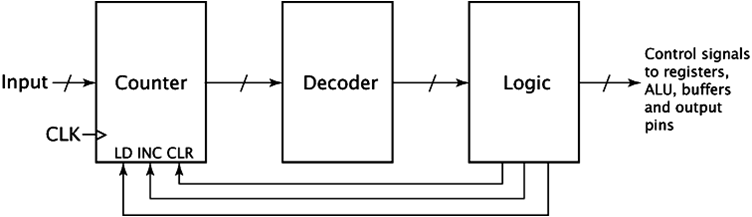
\includegraphics[scale=0.4]{GenericControlUnit}
  \end{center}
\end{frame}

\begin{frame}{VSCPU control unit}
  \begin{center}
    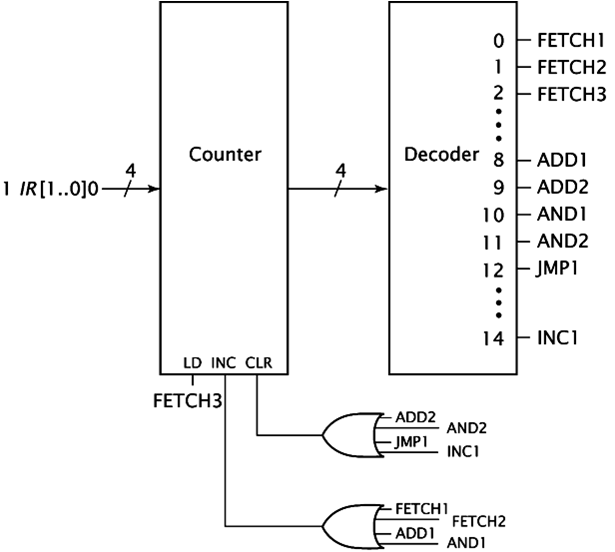
\includegraphics[scale=0.4]{VSCPUControlUnit}
  \end{center}
\end{frame}

\begin{frame}{VSCPU control signals}
  \begin{center}
    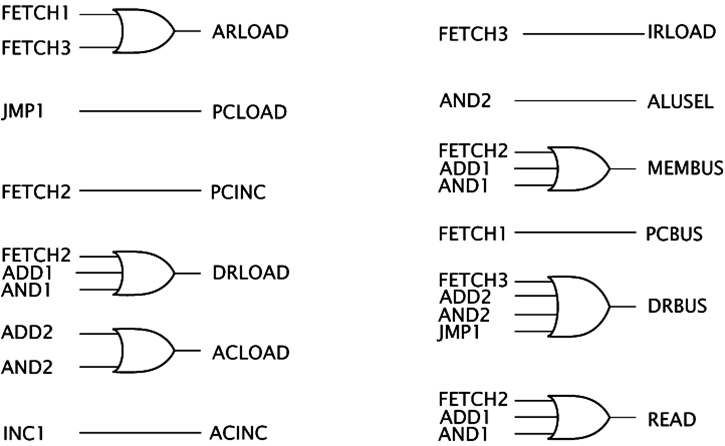
\includegraphics[scale=0.4]{ControlSignals}
  \end{center}
\end{frame}

\end{document}
